\begin{document}

% =======================================================================================
%\cleardoublepage % Forces the first chapter to start on an odd page so it's on the right

% =======================================================================================
%                                   PREAMBLE
% =======================================================================================
\coverpage{\TITLE}{\SUBTITLE}{\AUTHOR}{\DATE}{\SUBJECT}
%----------------------------------------------------------------------------------------
\newpage
\fpage
\newpage

\tableofcontents


\part{Introduction}
\chapter{General Descriptions}
Lung cancer is a disease characterized by the uncontrolled growth of abnormal cells in the tissues of the lungs. These abnormal cells can form tumors that interfere with the normal functioning of the lungs, such as breathing and oxygen exchange. Lung cancer is one of the leading causes of cancer-related deaths worldwide due to its high prevalence and often late-stage diagnosis.

\section{How does Lung Cancer develop?}
\begin{remark}
Lung cancer \cite{li2024gut} typically begins in the cells lining the airways. These cells undergo genetic mutations that cause them to grow uncontrollably and lose their normal function. Over time, these cells can invade surrounding tissues and spread to other parts of the body, a process known as metastasis \cite{shi2024mechanism}.
\end{remark}

\section{Global Impact}
\begin{outline}
Lung cancer has a significant global impact \cite{ramamoorthy2024assessing}, with millions of new cases and deaths reported annually. It is more common in regions with high smoking rates and industrial exposure. Early detection and preventive measures such as smoking cessation programs can greatly reduce the burden of this disease.
\end{outline}

\begin{figure}[h!]
    \centering
    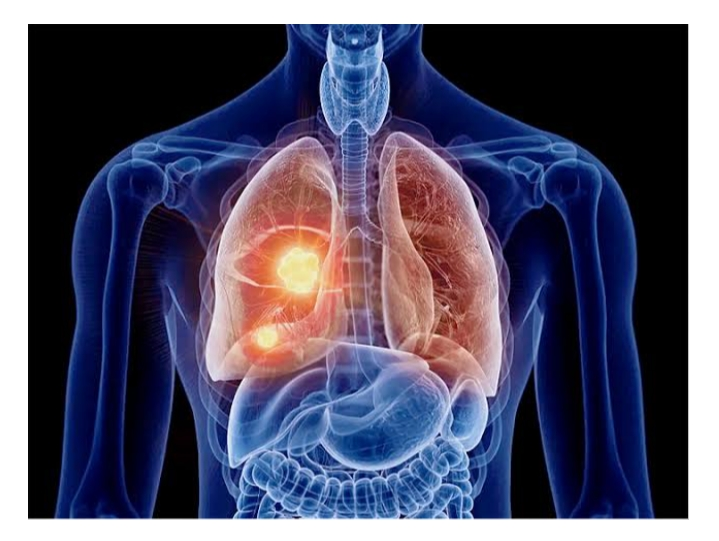
\includegraphics[width= 0.85\linewidth]{images/lung_c.jpeg}
    \caption{Lung cancer}
    \label{fig:enter-label}
\end{figure}

\chapter{Types of Lung Cancer}
There are two main types of lung cancer:
\begin{outline}
\begin{itemize}
    \item \textcolor{red}{Small Cell Lung Cancer} (SCLC)
    \item \textcolor{red}{Non Small Cell Lung Cancer} (NSCLC)    
\end{itemize}
\end{outline}
\section {Small Cell Lung Cancer (SCLC)}

SCLC is a fast-growing cancer that spreads much more quickly than other types of lung cancer. In most people with SCLC, the cancer has already spread beyond the lungs at the time it is diagnosed. Unfortunately, for most people the cancer will return at some point. SCLC are also classed as \textcolor{red}{neuroendocrine tumours} (NETs). Neuroendocrine tumours are rare tumours that develop in cells of the \textcolor{red}{neuroendocrine system}. In small cell lung cancer, the tumour starts in the \textcolor{red}{neuroendocrine cells} of the lung.

\begin{remark}
Almost all cases of small cell lung cancer are due to cigarette smoking. Around \textcolor{red}{15 to 20} out of every 100 lung cancers diagnosed are this type. 
\end{remark}

There are two different types of small cell lung cancer:
\begin{outline}
\begin{itemize}
    \item \textcolor{red}{small cell carcinoma} (also called \textcolor{red}{oat cell carcinoma})
    \item \textcolor{red}{combined small cell carcinoma}.
\end{itemize}
\end{outline}
\begin{remark}
The types of small cell lung cancer are named for the kinds of cells found in the cancer and how the cells look when viewed under a microscope. 
\end{remark}

\section{Non Small Cell Lung Cancer (NSCLC)} 
This type of cancer usually grows and spreads to other parts of the body more slowly than small cell lung cancer does. Around \textcolor{red}{80 to 85} out of 100 lung cancers are non small cell lung cancer (NSCLC). There are three different types of NSCLC:
\begin{outline}
\begin{itemize}
    \item \textcolor{red}{Adenocarcinoma}
    \item \textcolor{red}{Squamous cell carcinoma}
    \item \textcolor{red}{Large cell carcinoma}
\end{itemize}
\end{outline}

\begin{highlight}
\begin{enumerate}
    \item \textbf{Adenocarcinoma} A form of NSCLC often found in an outer area of the lung. It develops in the cells of epithelial tissues, which line the cavities and surfaces of the body and form glands.

    \item \textbf{Large cell carcinoma} A form of NSCLC usually found in the center of the lung next to an air tube (bronchus).

    \item \textbf{Squamous cell carcinoma} A form of NSCLC that can occur in any part of the lung and tends to grow and spread faster than adenocarcinoma or squamous cell carcinoma.
\end{enumerate}
\end{highlight}


\begin{figure}[ht!]
    \centering
    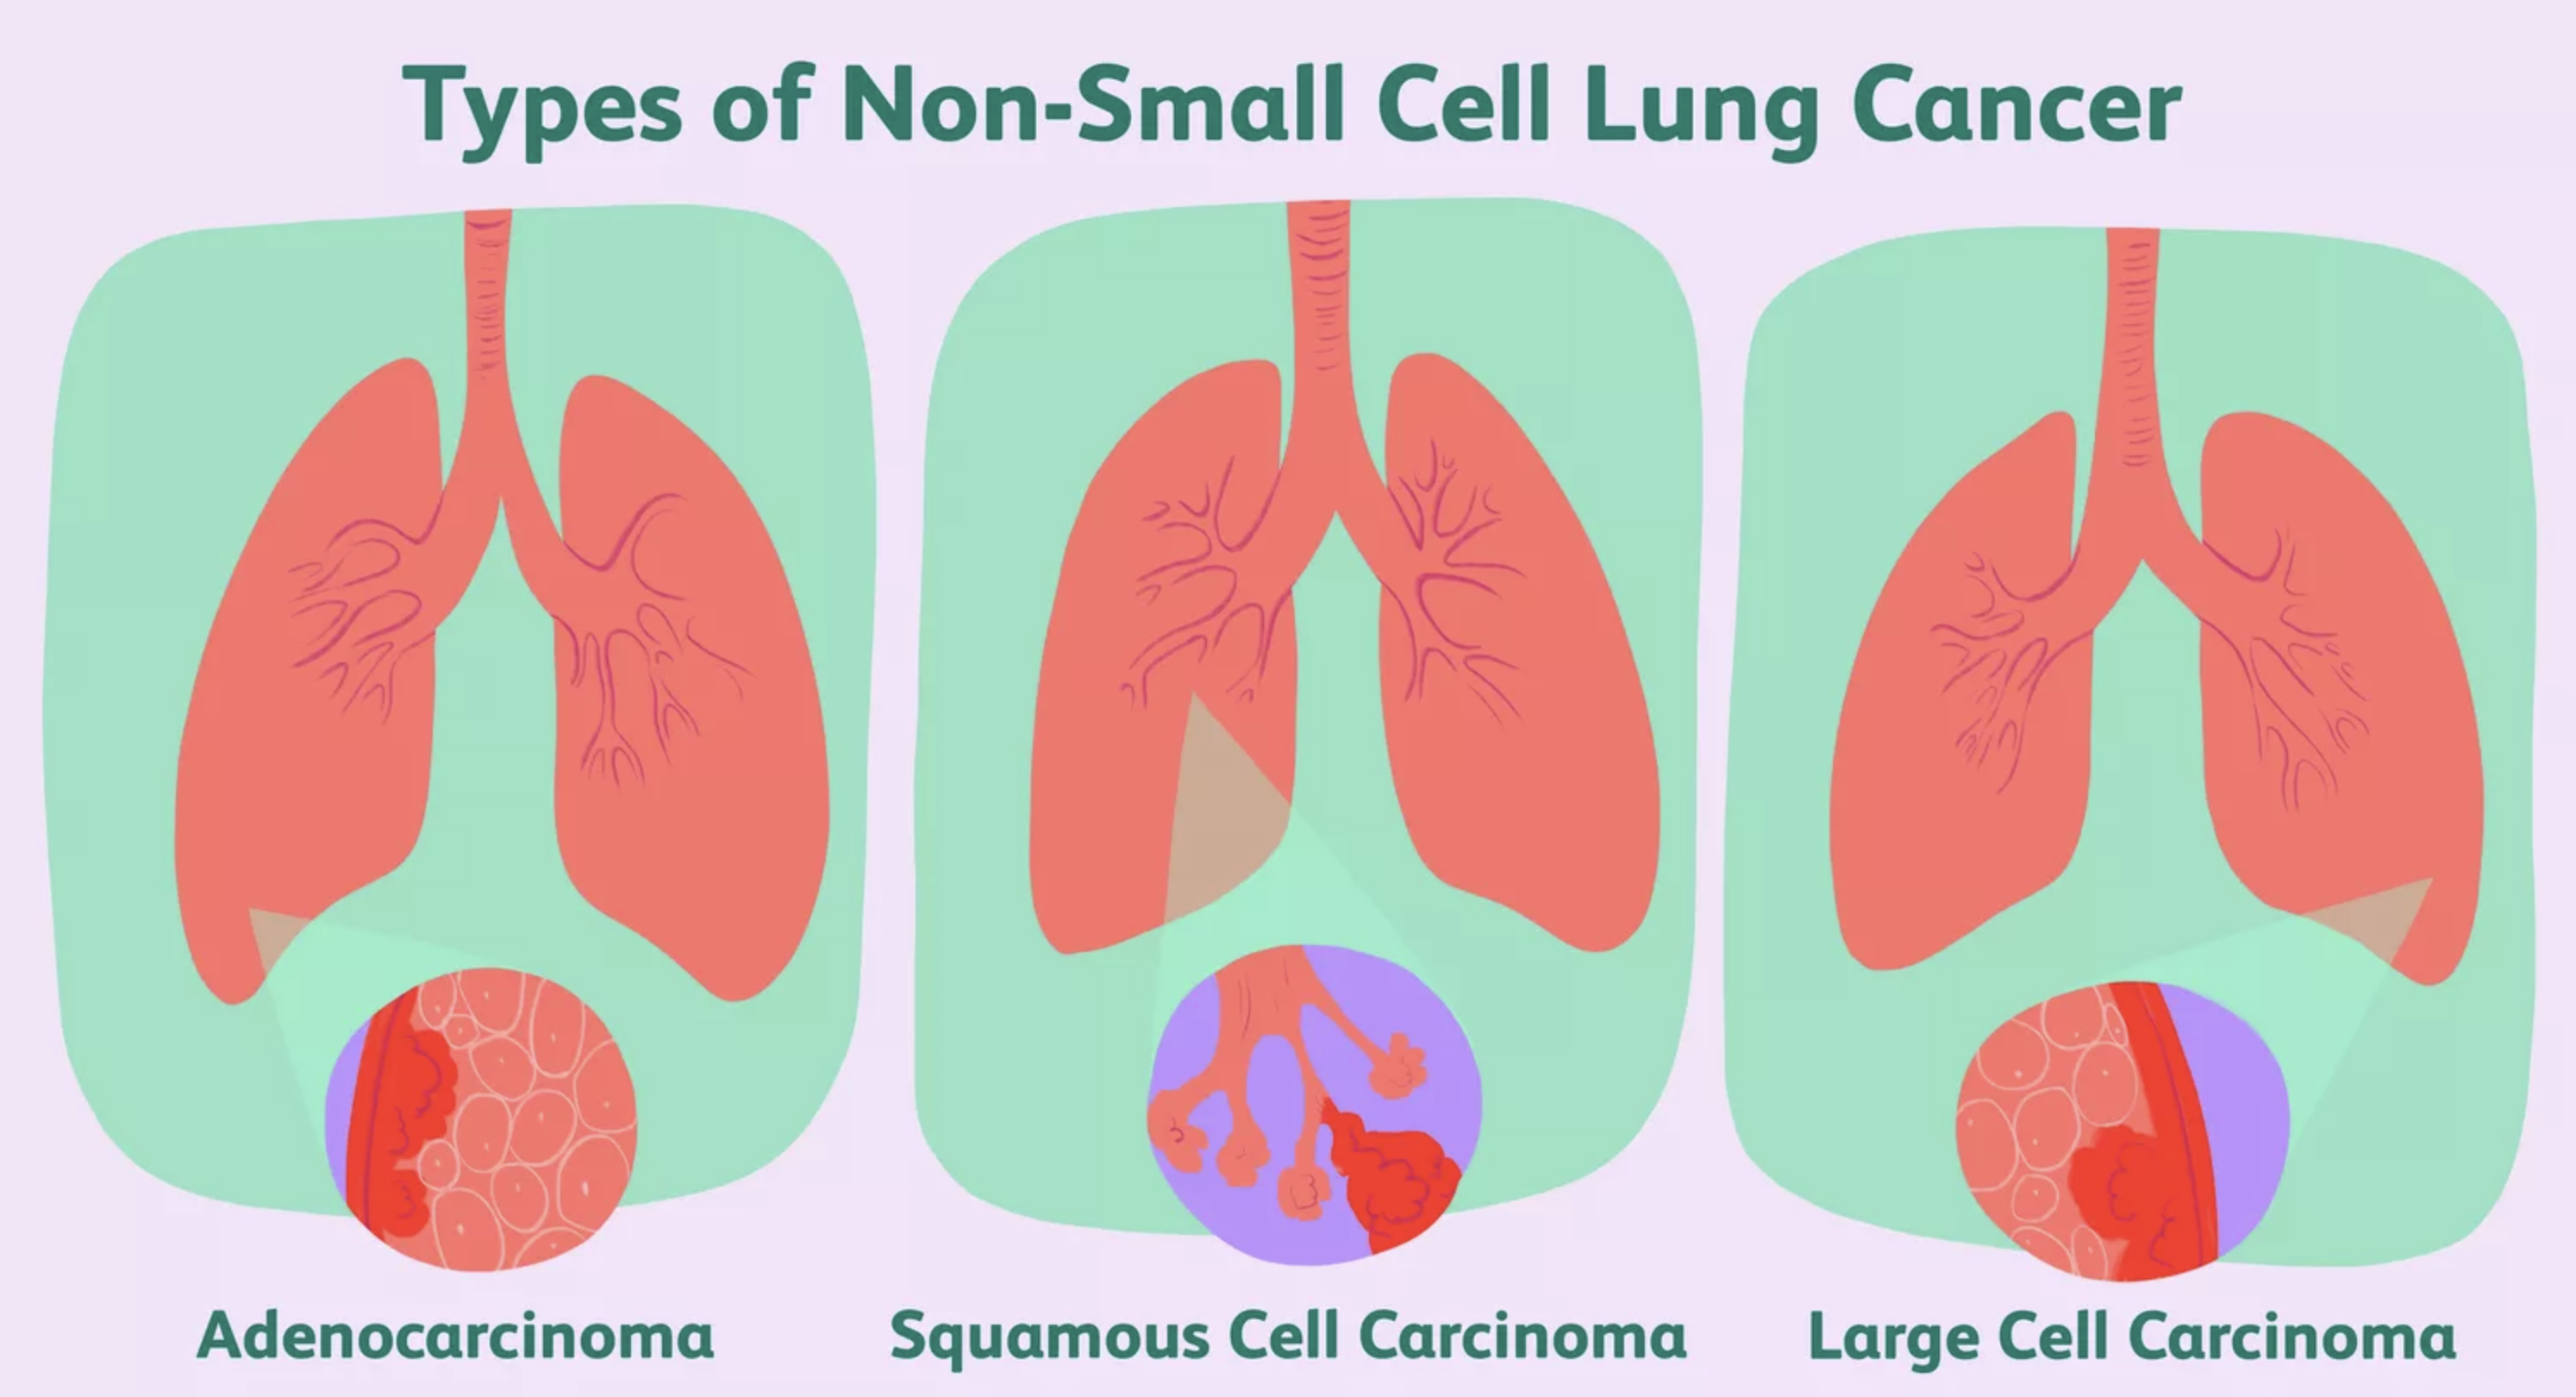
\includegraphics[width=\linewidth]{images/Non_small_cell_lung_cancer.png}
    \caption{Types of Non-Small cell Lung Cancer}
\end{figure}

\section{Other cancers affecting the lungs} 
\begin{remark}
There are other types of tumors found in the lung. They are rare. Examples are:- \textcolor{red}{\textbf{Salivary gland type tumors, Lung sarcoma, Lung lymphoma }}.
\end{remark}

Now lets have a look in the given diagram about percentage of different types of lung cancer:

\begin{figure}[h!]
    \centering
    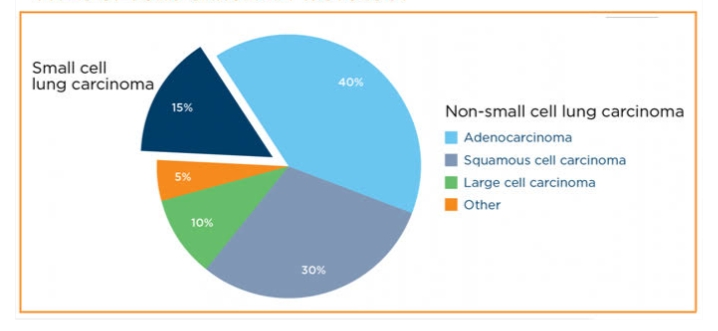
\includegraphics[width=0.7\linewidth]{images/percentage_of_lc.jpeg}
    \caption{Percentage of different types of lung cancer}
    \label{fig:types-label}
\end{figure}


\chapter{Stages of Lung Cancer}
The staging of lung cancer is crucial for determining the extent of the disease and guiding the appropriate treatment plan. Lung cancer staging is generally based on the size of the tumor, its location, and whether it has spread to nearby lymph nodes or other parts of the body.

\section{Stages of Non-Small Cell Lung Cancer (NSCLC)}
Non-Small Cell Lung Cancer (NSCLC) is classified into the following stages

\begin{itemize}
    \item \textbf{Stage 0 (In Situ)} The cancer is localized and confined to the inner lining of the lungs. At this stage, the tumor has not invaded deeper tissues or spread to other areas.
    \item \textbf{Stage I} The tumor is small (less than 4 cm) and limited to the lung, without spreading to lymph nodes.
    \item \textbf{Stage II} The tumor may be larger or have spread to nearby lymph nodes or tissues, such as the chest wall or diaphragm.
    \item \textbf{Stage III} The cancer has spread to more distant lymph nodes or other nearby structures, such as the heart or trachea.
    \item \textbf{Stage IV} The cancer has \textcolor{red}{metastasized}, meaning it has spread to distant parts of the body, such as the liver, brain, or bones.
\end{itemize}

\section{Stages of Small Cell Lung Cancer (SCLC)} 
Small Cell Lung Cancer (SCLC) is typically classified into two broad stages due to its aggressive nature:

\begin{itemize}
    \item \textbf{Limited Stage} The cancer is confined to one side of the chest, involving only one lung and nearby lymph nodes.
    \item \textbf{Extensive Stage} The cancer has spread to the other lung, distant lymph nodes, or other parts of the body.
\end{itemize}

\section{TNM Classification} 
The \textcolor{red}{TNM} system is also commonly used to describe lung cancer stages:
\begin{itemize}
    \item \textbf{T (Tumor)}  Refers to the size and extent of the primary tumor.
    \item \textbf{N (Nodes)} Indicates whether cancer has spread to nearby lymph nodes.
    \item \textbf{M (Metastasis)} Describes whether the cancer has spread to distant parts of the body.
\end{itemize}

Understanding the stage of lung cancer helps oncologists design personalized treatment plans; including surgery, \textcolor{red}{chemotherapy}, \textcolor{red}{radiation therapy}, or \textcolor{red}{targeted therapies}. Early-stage detection offers a higher chance of successful treatment, while advanced stages require a more comprehensive approach.


\part{Prevention}
\chapter{Symptoms of Lung Cancer}
Lung cancer symptoms may vary depending on the type, stage, and location of the cancer. Common symptoms include:

\begin{highlight}
\begin{itemize}
    \item Persistent cough that does not go away or worsens over time.
    \item Coughing up blood (\textcolor{red}{hemoptysis}) or rust-colored \textcolor{red}{sputum}.
    \item Shortness of breath (\textcolor{red}{dyspnea}).
    \item Chest pain or discomfort, especially when breathing deeply, coughing, or laughing.
    \item \textcolor{red}{Hoarseness} or changes in voice.
    \item Unexplained weight loss or loss of appetite.
    \item \textcolor{red}{Fatigue} or feeling weak.
    \item Frequent infections, such as \textcolor{red}{bronchitis} or \textcolor{red}{pneumonia} .
    \item \textcolor{red}{Wheezing} or noisy breathing.
    \item \textcolor{red}{Swelling} in the face, neck, or upper body (\textcolor{red}{superior vena cava syndrome}).
    \item Bone pain or \textcolor{red}{tenderness} (if cancer has spread to bones).
    \item \textcolor{red}{Neurological symptoms}, such as headache, dizziness, or numbness, if the cancer has spread to the brain.
\end{itemize}
\end{highlight}
\begin{remark}
Note that many of these symptoms can also be caused by other conditions. It is important to consult a healthcare provider for an accurate diagnosis.
\end{remark}
\begin{figure}[h!]
    \centering
    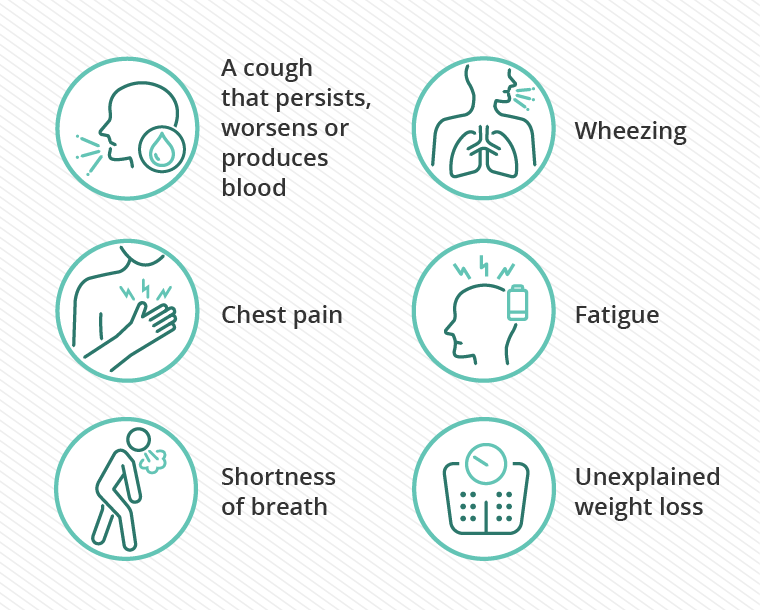
\includegraphics[width= 0.675\linewidth]{images/Lung-Cancer-Symptoms-DT.png}
    \caption{Symptoms of lung cancer}
    \label{fig:symptoms}
\end{figure}

\newpage

\chapter{Diagnosis and Treatment}
\begin{remark}
Early and accurate diagnosis of lung cancer is crucial for effective treatment and management. According to \cite{deng2024prospects} the diagnostic process typically involves a combination of \textcolor{red}{imaging studies} , \textcolor{red}{laboratory tests} , and \textcolor{red}{biopsy procedures} to confirm the presence of cancer and determine its type and stage.
\end{remark}

\section{Imaging Tests} 
Imaging studies are often the first step in diagnosing lung cancer. These tests help visualize abnormalities in the lungs and surrounding tissues.

\begin{highlight}
\begin{itemize}
    \item \textbf{Chest X-ray} Often the initial test used to detect unusual masses or spots in the lungs\cite{kalkeseetharaman2024bird}.
    \item \textbf{Computed Tomography (CT) Scan} Provides detailed cross-sectional images of the lungs and chest, helping to identify the size, shape, and location of tumors\cite{hendrick2024benefit}.
    \item \textbf{Positron Emission Tomography (PET) Scan} Helps determine if the cancer has spread by detecting areas of increased metabolic activity.
    \item \textbf{Magnetic Resonance Imaging (MRI)} Used in specific cases, especially when there is a suspicion of cancer spreading to the brain or spinal cord\cite{li2024application}.
\end{itemize}
\end{highlight}

\section{Laboratory Tests}
Lab tests analyze blood, sputum, or other samples to detect cancer-related abnormalities.

\begin{highlight}
\begin{itemize}
    \item \textbf{Sputum Cytology} \cite{wen2024methylated}Examines mucus produced by coughing for the presence of cancer cells, particularly in central lung tumors.
    \item \textbf{Blood Tests} While not diagnostic for lung cancer, blood tests can help assess overall health and detect markers that may indicate cancer.
\end{itemize}
\end{highlight}

\section{Biopsy Procedures} 
A biopsy involves the removal of tissue or fluid samples for microscopic examination. It is the definitive method for diagnosing lung cancer and determining its type:

\begin{highlight}
\begin{itemize}
    \item \textbf{Bronchoscopy} \cite{rozman2024interventional}A thin, flexible tube is inserted through the nose or mouth to examine the airways and collect tissue samples.
    \item \textbf{Needle Aspiration (Fine Needle Aspiration or Core Biopsy)} \cite{lee2024additional} A needle is used to extract cells or tissue from the lung or lymph nodes, often guided by imaging techniques.
    \item \textbf{Thoracentesis} \cite{dahlberg2024thoracentesis} Removes fluid from around the lungs (pleural effusion) to check for cancer cells.
    \item \textbf{Surgical Biopsy} \cite{mahuron2024applications} Performed when other methods are inconclusive; includes procedures like \textcolor{red}{thoracoscopy} or \textcolor{red}{thoracotomy}.
\end{itemize}
\end{highlight}

\section{Molecular and Genetic Testing}
\begin{outline}
Advances in cancer treatment have led to the use of molecular and genetic testing of tumor samples\cite{kanasaki2024upfront}. These tests identify specific mutations (e.g., \textcolor{red}{EGFR, ALK, KRAS}) and biomarkers that can guide personalized treatment, such as \textcolor{red}{targeted therapies} or \textcolor{red}{immunotherapies}\cite{li2024targeted}.
\end{outline}

\section{Staging Tests} 
Once a lung cancer diagnosis is confirmed, staging tests are conducted to determine the extent of the disease. These may include additional imaging studies like \textcolor{red}{bone scans}, \textcolor{red}{PET-CT}, or \textcolor{red}{MRI}, and lymph node evaluation using \textcolor{red}{mediastinoscopy} or \textcolor{red}{endobronchial ultrasound (EBUS)}\cite{de2024future}.

\begin{remark}
Accurate diagnosis and staging enable oncologists to develop tailored treatment plans, improving outcomes and quality of life for patients.
\end{remark}

\part{Statistics}
\chapter{Management and Treatment}
\begin{remark}
The management and treatment of lung cancer vary depending on the type, stage, and overall health of the patient. Advances in medical technology and understanding of the disease have greatly improved treatment options, offering patients personalized and targeted approaches.
\end{remark}

\section{Surgical Options}
According to \cite{hoy2019surgical}, surgery is often recommended for early-stage non-small cell lung cancer (NSCLC) if the cancer is localized and the patient is healthy enough to undergo the procedure. Common surgical procedures include:
\begin{highlight}
\begin{itemize}
    \item \textbf{Lobectomy:} Removal of the affected lobe of the lung.
    \item \textbf{Pneumonectomy:} Removal of an entire lung in cases of extensive disease.
    \item \textbf{Segmentectomy or Wedge Resection:} Removal of a smaller portion of the lung, typically for patients unable to tolerate more extensive surgery.
\end{itemize}
\end{highlight}

\section{Radiation Therapy}
According to \cite{de2013state}, Radiation therapy uses high-energy rays to destroy cancer cells. It can be used in conjunction with surgery or as a standalone treatment in cases where surgery isn’t an option. Techniques include:
\begin{highlight}
\begin{itemize}
    \item \textbf{External Beam Radiation Therapy (EBRT):} Targets cancer cells from outside the body.
    \item \textbf{Stereotactic Body Radiation Therapy (SBRT):} A precise and focused form of radiation used for small tumors.
\end{itemize}
\end{highlight}

\section{Chemotherapy}
\begin{outline}
According to \cite{ihde1992chemotherapy}, Chemotherapy involves the use of drugs to kill cancer cells or stop their growth. It is commonly used in advanced stages of both NSCLC and small cell lung cancer (SCLC) and may be combined with other treatments. Commonly used drugs include cisplatin and carboplatin.
\end{outline}

\section{Targeted Therapy}
According to \cite{mayekar2017current}, Targeted therapy focuses on specific genetic mutations or proteins that drive cancer growth. It is most effective in NSCLC with identifiable mutations, such as: 
\begin{highlight}
\begin{itemize}
    \item \textbf{EGFR inhibitors} (e.g., erlotinib, gefitinib)
    \item \textbf{ALK inhibitors} (e.g., crizotinib, alectinib)
    \item \textbf{ROS1 inhibitors}
\end{itemize}
\end{highlight}

\section{Immunotherapy}
\begin{outline}
According to \cite{steven2016immunotherapy}, Immunotherapy helps the immune system recognize and attack cancer cells. Drugs like immune checkpoint inhibitors (e.g., pembrolizumab, nivolumab) have shown promise, particularly in advanced NSCLC.
\end{outline}

\section{Palliative Care}
\begin{outline}
Palliative care focuses on improving quality of life by managing symptoms such as pain, breathlessness, and fatigue. It is an essential part of treatment for advanced lung cancer and may include medications, counseling, and support for patients and families, according to \cite{ferrell2011palliative}.
\end{outline}

\section{Lifestyle and Supportive Measures}
\begin{outline}
Patients are encouraged to adopt healthy habits, such as quitting smoking and eating a balanced diet, to improve overall outcomes. Emotional and psychological support, including therapy and support groups, plays a critical role in the treatment journey, according to \cite{heredia2023effectiveness}.
\end{outline}

\section{Future Directions}
\begin{remark}
Emerging therapies, including gene therapy and personalized medicine, hold promise for the future of lung cancer treatment. Ongoing research aims to improve survival rates and quality of life for patients.
\end{remark}

An integrated approach combining different therapies tailored to each patient's needs is crucial for effective lung cancer management.

\chapter{Statistics of Lung Cancer}
\section{Global Statistics}
\begin{remark}
According to \cite{jemal2011global}, lung cancer is one of the most commonly diagnosed cancers worldwide and remains a leading cause of cancer-related deaths. 
\end{remark}
According to the latest estimates by the \textbf{World Health Organization (WHO)} and the \textbf{Global Cancer Observatory (GLOBOCAN)}:
\begin{highlight}
\begin{itemize}
    \item Lung cancer accounted for approximately \textbf{2.2 million new cases} and over \textbf{1.8 million deaths} globally in 2020.
    \item It represents about \textbf{11.4\% of all new cancer cases} and \textbf{18\% of all cancer deaths}, making it the most fatal cancer globally.
    \item The incidence rate is significantly higher in \textbf{men}, with nearly \textbf{1.4 million cases}, compared to approximately \textbf{770,000 cases in women}.
\end{itemize}
\end{highlight}

Geographically, the highest incidence rates are observed in:
\begin{highlight}
\begin{itemize}
    \item \textbf{Eastern Europe} and \textbf{Eastern Asia}: High smoking prevalence drives these rates.
    \item \textbf{North America} and \textbf{Western Europe}: Advanced diagnostics contribute to the detection of cases, including early stages.
\end{itemize}
\end{highlight}
\begin{figure}[h!]
    \centering
    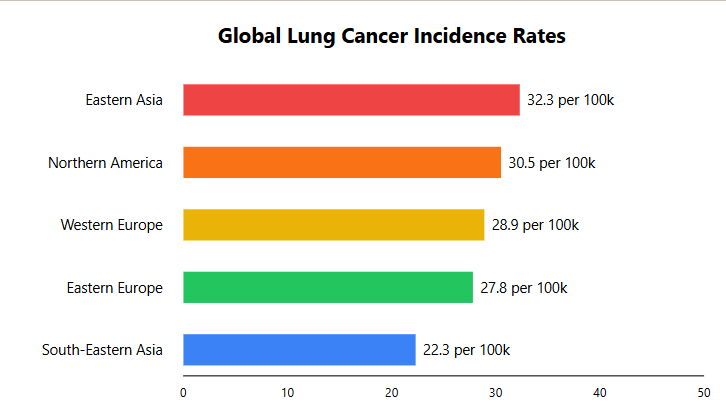
\includegraphics[width=0.8\textwidth]{images/lunc cancer global.png}
    \caption{Charts illustrating global lung cancer statistics}
    \label{fig:lung_stats}
\end{figure}
\newpage
\section{Lung Cancer in India}
Lung cancer is a significant public health challenge in India, with the following key statistics, according to \cite{singh2021lung}:
\begin{highlight}
\begin{itemize}
    \item \textbf{Incidence:} Lung cancer ranks among the \textbf{top three cancers in men} and is increasingly common in women. In 2020, there were approximately \textbf{72,000 new cases} of lung cancer in India.
    \item \textbf{Mortality:} Lung cancer accounted for nearly \textbf{66,000 deaths}, making it a leading cause of cancer-related fatalities in the country.
    \item \textbf{Trends:} While smoking remains the primary cause, rising pollution levels, exposure to industrial \textbf{carcinogens}, and passive smoking are contributing factors. Non-smokers constitute a growing proportion of cases, especially among women.
\end{itemize}
\end{highlight}
\begin{figure}[h!]
    \centering
    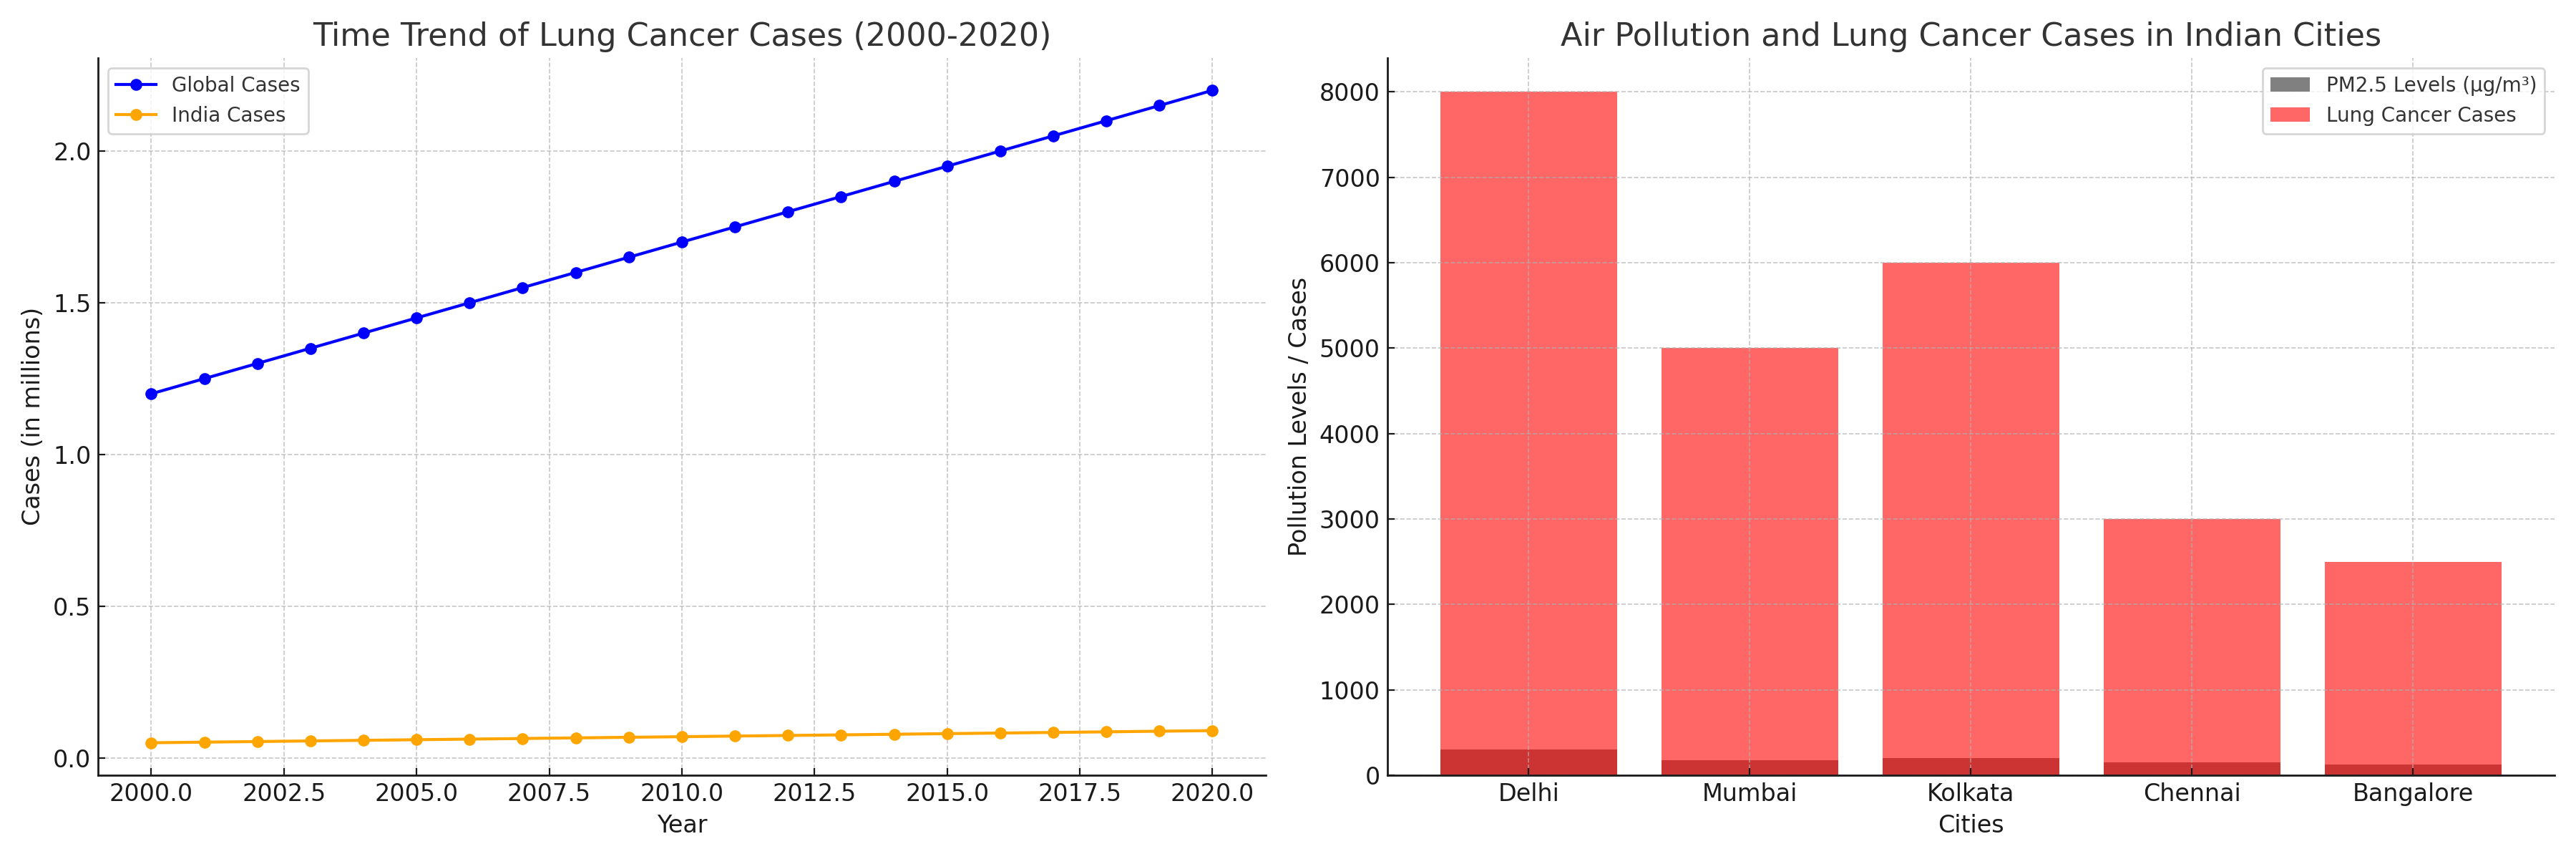
\includegraphics[width=\textwidth]{images/lung_cancer_additional_charts.png}
    \caption{Charts illustrating global and Indian lung cancer statistics}
    \label{fig:lung_stats_2}
\end{figure}
\section{Gender Distribution of Lung Cancer in India}
\begin{remark}
Lung cancer incidence in India shows significant variation between genders. 
\end{remark} 
Key observations are outlined below:

\subsection{Incidence Among Men and Women}

According to the study published in \cite{meza2015lung}
\begin{outline}
\begin{itemize}
    \item \textbf{Men:} Lung cancer remains one of the leading cancers among men, accounting for approximately \textbf{70-75\% of total cases}. This high prevalence is primarily attributed to smoking (bidi and cigarette use), occupational exposure to carcinogens, and outdoor air pollution.
    \item \textbf{Women:} Though less common, lung cancer cases among women are increasing due to factors like \textbf{indoor air pollution} from biomass fuel, passive smoking, and exposure to environmental pollutants. Non-smoking-related cases constitute a significant proportion.
\end{itemize}
\end{outline}

\subsection{Risk Factors in Gender Distribution}
In accordance to the study published in \cite{huang2022distribution}
\begin{outline}
\begin{itemize}

    \item \textbf{Men:} Smoking remains the dominant factor, contributing to the majority of cases. Occupational hazards and outdoor air pollution also play significant roles.
    \item \textbf{Women:} A large proportion of women diagnosed with lung cancer are \textbf{non-smokers}. Indoor air pollution and passive smoking are major contributors.
\end{itemize}
\end{outline}

\subsection{Trends Over Time}
According to \cite{jemal2001recent}:
\begin{outline}
\begin{itemize}

    \item A \textbf{decline in smoking rates among men} has contributed to a slower increase in lung cancer cases in this group.
    \item An \textbf{increase in non-smoking-related cases among women} is evident, largely due to environmental and lifestyle changes.
\end{itemize}
\end{outline}

\begin{figure}[h!]
    \centering
    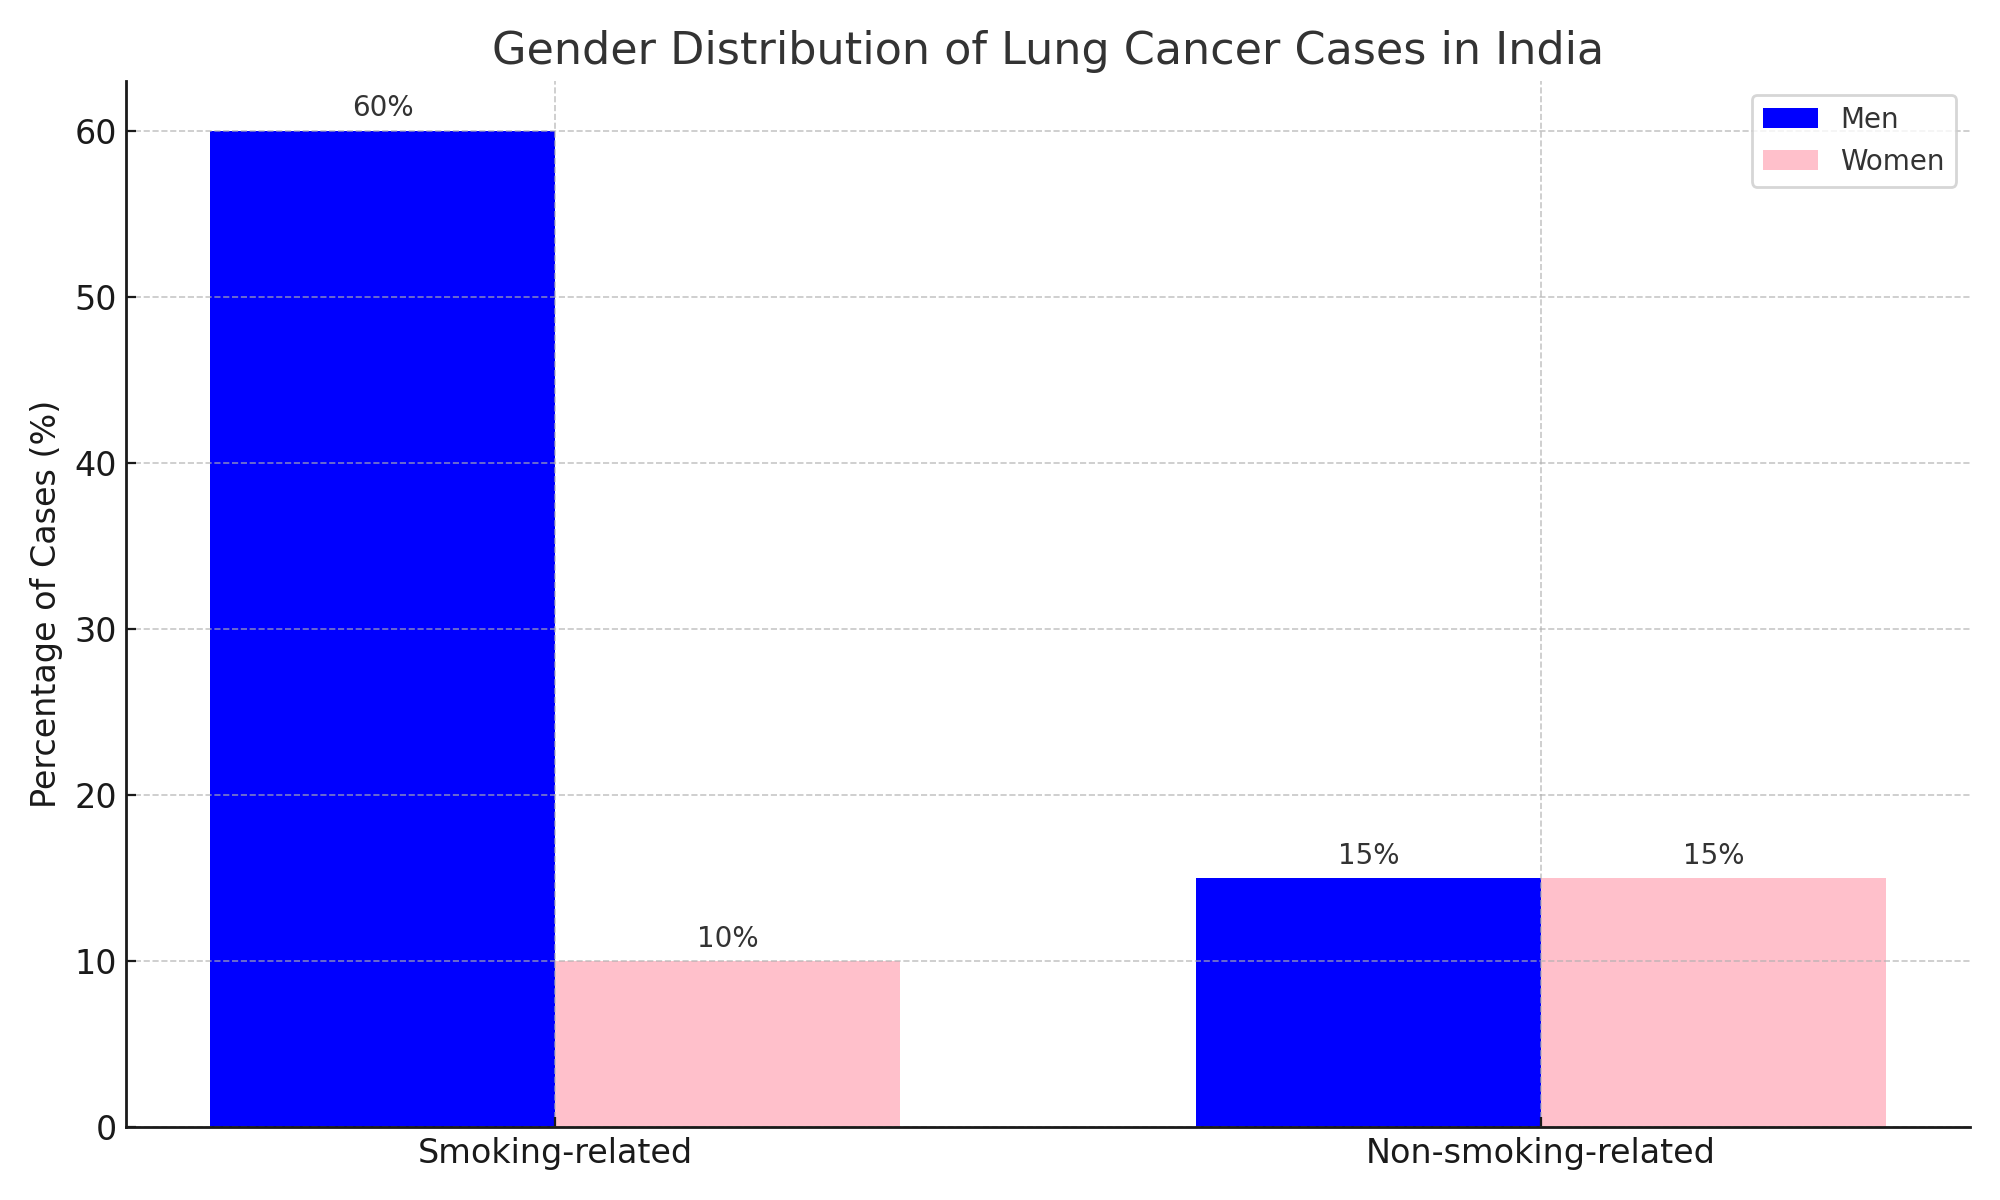
\includegraphics[width=0.8\textwidth]{images/lung_cancer_gender_distribution_chart.png}
    \caption{Gender distribution of lung cancer cases in India}
    \label{fig:gender_distribution}
\end{figure}

\section{Risk Factors Contributing to the Statistics}
\begin{highlight}
\begin{enumerate}
    \item \textbf{Smoking:}
    \begin{itemize}
        \item Globally, over \textbf{80\% of lung cancer cases} are attributed to smoking. In India, a large proportion of men smoke tobacco, while \textbf{bidi smoking} and \textbf{chewing tobacco} further exacerbate the risk.
    \end{itemize}
    \item \textbf{Air Pollution:}
    \begin{itemize}
        \item India faces some of the world's worst air quality, with particulate matter \textbf{(PM2.5)} exposure significantly increasing lung cancer risks, particularly in urban areas like \textbf{Delhi} and\textbf{ Mumbai}.
    \end{itemize}
    \item \textbf{Occupational Hazards:}
    \begin{itemize}
        \item Prolonged exposure to asbestos, arsenic, and other carcinogens in industrial settings has raised lung cancer incidence in India.
    \end{itemize}
\end{enumerate}
\end{highlight}

As stated in the study performed in \cite{akhtar2017risk}.

\section{Global and National Efforts}
\begin{remark}
To combat lung cancer, global initiatives focus on smoking cessation, air quality improvement, and early diagnosis. 
\end{remark}
In India, according to \cite{leiter2023global}:
\begin{highlight}
\begin{itemize}
    \item The \textbf{National Program for Prevention and Control of Cancer, Diabetes, Cardiovascular Diseases, and Stroke (NPCDCS)} supports early screening and treatment.
    \item Anti-tobacco campaigns and regulations have contributed to reducing smoking prevalence.
    \item Awareness programs targeting pollution and occupational safety are gaining momentum.
\end{itemize}
\end{highlight}

\section{The Path Forward}
\begin{remark}
Despite advancements, the burden of lung cancer remains high. Efforts to curb smoking, mitigate pollution, and improve healthcare access are critical to addressing the challenges globally and in India. Comprehensive data collection and research will also help shape effective policies and interventions.
\end{remark}

\part{Appendices}
\listoffigures
\newpage\printbibliography[title = {References}]

\end{document}